% (c) 2015 Daniele Zambelli daniele.zambelli@gmail.com

\section{TODO}

\section{Esercizi}

\subsection{Esercizi dei singoli paragrafi}

\subsubsection*{\numnameref{sec:01_}}

\begin{esercizio}
\label{ese:D.19}
testo esercizio
\end{esercizio}

\begin{esercizio}\label{ese:03.1}
Consegna:
 \begin{enumeratea}
  \item  
 \end{enumeratea}
\end{esercizio}




\subsection{Esercizi}

Calcola il valore dei seguenti valori assoluti:
\begin{enumerate}
\item $|-2|=\dots$
\item $|+7|=\dots$
\item $|3-7|=\dots$
\item $|5-\frac{1}{3}|=\dots$
\item $|\sqrt{2}-\sqrt{6}|=\dots$
\item $|\sqrt{3}-2|=\dots$
\end{enumerate}

Completa come nell'esempio:
$$
|2x|=
        \left\lbrace 
        \begin{array}{lcl}
        2x & \text{se}& x\geq 0\\
        -2x & \text{se}& x< 0\\
        \end{array}
        \right.
$$

\begin{enumerate}
        \item 
        $$
        |4x|=
        \left\lbrace 
        \begin{array}{lcl}
        \dots & \text{se}& x\geq\dots\\
        \dots & \text{se}& x<\dots\\
        \end{array}
        \right.
        $$
        \item 
        $$
        |-2x|=
        \left\lbrace 
        \begin{array}{lcl}
        \dots & \text{se}& x\geq\dots\\
        \dots & \text{se}& x<\dots\\
        \end{array}
        \right.
        $$
        \item 
        $$
        |x-3|=
        \left\lbrace 
        \begin{array}{lcl}
        x-3 & \text{se}& x\geq\dots\\
        \dots & \text{se}& x<\dots\\
        \end{array}
        \right.
        $$
        \item 
        $$
        |x^2-2x|=
        \left\lbrace 
        \begin{array}{lcl}
        \dots & \text{se}& x\leq\dots \vee x\geq\dots\\
        \dots & \text{se}& \dots <x<\dots\\
        \end{array}
        \right.
        $$
        \item 
        $$
        |7-2x|=
        \left\lbrace 
        \begin{array}{lcl}
        \dots & \text{se}& x\geq\dots\\
        \dots & \text{se}& x<\dots\\
        \end{array}
        \right.
        $$
        \item 
        $$
        |x^2-6x+8|=
        \left\lbrace 
        \begin{array}{lcl}
        \dots & \text{se}& x\leq\dots \vee x\geq\dots\\
        \dots & \text{se}& \dots <x<\dots\\
        \end{array}
        \right.
        $$
        \item 
        $$
        |\frac{x-1}{2x}|=
        \left\lbrace 
        \begin{array}{lcl}
        \frac{x-1}{2x} & \text{se}& x\leq\dots \vee x\geq\dots\\
        \dots & \text{se}& \dots <x<\dots\\
        \end{array}
        \right.
        $$
\end{enumerate}
Interpretazione di grafici:
\begin{enumerate}
\item Quale delle seguenti figure rappresenta il grafico della funzione 
$y=|x-4|$?

\begin{figure}[h]
\begin{inaccessibleblock}[TODO]
\centering
\includegraphics[width=0.9\linewidth]{img/imm6} %[scale=0.35]{img/fig001.png}
\end{inaccessibleblock}
% \caption{Retta}
\label{fig:abs_imm6}
\end{figure}
% \begin{figure}[h]
%         \centering
%         \includegraphics[width=0.9\linewidth]{imm6}
%         %\caption{}
%         \label{fig:imm1}
% \end{figure}
\end{enumerate}
Traccia il grafico delle seguenti funzioni come nell'esempio:
$$y=|x^2-4|$$
\begin{tabular}{cc}
\begin{tabular}{|c|c|}
        \hline
        x & y \\
        \hline
        0 & 4 \\
        \hline  
        -1 & 3 \\
        \hline
        1 & 3 \\
        \hline
        -2 & 0 \\
        \hline
        2 & 0 \\
        \hline
        -3 & 5 \\
        \hline
        3 & 5 \\
        \hline                                                  
\end{tabular}   
&

\begin{inaccessibleblock}[TODO]
\centering
\includegraphics[width=0.5\linewidth]{img/imm7} %[scale=0.35]{img/fig001.png}
\end{inaccessibleblock}
%       \includegraphics[width=0.5\linewidth]{imm7}
\\
\end{tabular}

\begin{enumerate}
        \item $y=|2x-1|$
        \item $y=|x+2|$
        \item $y=|x-1|$
        \item $y=2|x-1|$
        \item $y=\frac{|x-2|}{2}$
        \item $y=|3x|$
        \item $y=|x^2-3x+2|$
        \item $y=|x^2-1|$
\end{enumerate}
Equazioni del tipo $|P(x)|=k$\\
Esempi:
\begin{enumerate}
\item[a)] $|x^2-3|=0$, ricordando che $|x^2-3|=0$ se e solo se $x^2-3=0$, 
l'equazione ha come soluzioni $x=\pm\sqrt{3}$.
\item[b)] $|x^2-3|=-2$, impossibile perché il valore assoluto di un'espressione 
algebrica è sempre un numero non negativo.
\item[c)] $|2x-3|=2$, l'equazione equivale a:
$$2x-3=2 \vee 2x-3=-2$$
e quindi
$$x=\frac{5}{2}\vee x=\frac{1}{2}$$
\end{enumerate}
Risolvi le seguenti equazioni:

\begin{enumerate}
        \item $|x-3|=2$ \hfill $\left[ 1, 5\right] $
        \item $|x+1|=3$ \hfill $\left[ -4, 2\right] $
        \item $|x^2-6x+8|=0$ \hfill $\left[ 2, 4\right] $
        \item $\left| \frac{x-1}{2x}\right| =\frac{1}{4}$ \hfill $\left[ 
\frac{2}{3}, 2\right] $
                \item $|x^2-9|=-3$ \hfill $\left[impossibile \right] $
                \item $|x^4-x^2|=0$ \hfill $\left[ 0, \pm 1\right] $
                \item $|4x+3|=2$ \hfill $\left[ -\frac{3}{2}, -\frac{1}{4} 
\right] $
                \item $|x^2-6x+4|=4$ \hfill $\left[ 0, 2, 4 , 6 \right] $
                \item $|x^2-2x|=1$ \hfill $\left[ 1, 1+\sqrt{2} \right] $
                \item $|2x^3+6x-5|=-2$ \hfill $\left[ impossibile \right] $
                \item $\left| \frac{x^2-3x}{x+2}\right| =1$ \hfill $\left[ 2\pm 
\sqrt{6} \right] $
                \item $|x+3|=2$ \hfill $\left[ -1, -5 \right] $
\end{enumerate}



Equazioni del tipo $|A(x)|=|B(x)|$\\
Esempi:
\begin{enumerate}
        \item[a)] $|x^2-4|=|x-2|$, l'equazione equivale a
        $$x^2-4=x-2 \vee x^2-4=-(x-2)$$
        cioè:
        $$x^2-x-2=0 \vee x^2+x+6=0$$la prima equazione ha soluzioni $[-1, 2]$, 
la seconda $[-3, 2]$, pertanto le soluzioni dell'equazione di partenza sono 
$S=\left\lbrace -3, -1, 2\right\rbrace $.
        
        \item[b)] $|x^2-3|=-2$, impossibile perché il valore assoluto di 
un'espressione algebrica è sempre un numero non negativo.
        \item[c)] $|2x-3|=2$, l'equazione equivale a:
        $$2x-3=2 \vee 2x-3=-2$$
        e quindi
        $$x=\frac{5}{2}\vee x=\frac{1}{2}$$
\end{enumerate}

Risolvi le seguenti equazioni:

\begin{enumerate}
\item $\left| x-1\right| =\left| 2x-3\right| $ \hfill $\left[ \frac{4}{3}, 
2\right] $
\item $\left| x+1\right| =\left| 2x-1\right| $ \hfill $\left[ 0, 2\right] $
\item $\left| x^2-2x+3 \right| =\left| x-4 \right| $ \hfill $\left[ 
\frac{1\pm\sqrt{5}}{2}\right] $
\item $\left| x^2-x-5\right| =\left| x-2\right| $ \hfill $\left[ -1, 3, \pm 
\sqrt{7}\right] $
\item $\left| x+3\right| =\left| x\right| $ \hfill $\left[ -\frac{3}{2} \right] 
$
\item $\left| x^2-5x \right| =\left| x^2+2x \right| $ \hfill $\left[ 0, 
\frac{3}{2} \right] $
\item $\left| 3x+5\right| =\left| 2x+3\right| $ \hfill $\left[-2, -\frac{8}{5} 
\right] $
\item $\left| x+1\right| =\left| 2x\right| $ \hfill $\left[ -\frac{1}{3}, 1 
\right] $
\item $\left| x^3-6x\right| =\left| x^3-2x\right| $ \hfill $\left[ 0, \pm 2 
\right] $
\item $\left|\frac{x^2+1}{x}\right| =\left| 2x\right| $ \hfill $\left[ \pm 1 
\right] $
\item $\left| x^2-3x-10\right| =\left| x^2-4\right| $ \hfill $\left[-2, 
\frac{7}{2} \right] $
\end{enumerate}

Equazioni del tipo $|A(x)|=B(x)$\\
Esempi:
\begin{enumerate}
        \item[a)] $|x-3|=2x+2$, l'equazione equivale a risolvere:
        $$
        \left\lbrace 
        \begin{array}{l}
        x-3\geq 0 \\
        x-3=2x+2\\
        \end{array}
        \right.
        \vee
        \left\lbrace 
        \begin{array}{l}
        x-3< 0 \\
        -(x-3)=2x+2\\
        \end{array}
        \right.
        $$      

        cioè:
        $$
        \left\lbrace 
        \begin{array}{l}
        x\geq 3 \\
        x=-52\\
        \end{array}
        \right.
        \vee
        \left\lbrace 
        \begin{array}{l}
        x< 3 \\
        x=\frac{1}{3}\\
        \end{array}
        \right.
        $$
il primo sistema non ammette soluzione, pertanto la soluzione dell'equazione di 
partenza è $    x=\frac{1}{3}$.
\end{enumerate}

Risolvi le seguenti equazioni:

\begin{enumerate}
\item $\left| x+3 \right| =5x-2 $ \hfill $\left[ \frac{5}{4}\right] $
\item $\left| x-1 \right| =2x $ \hfill $\left[ \frac{1}{3}\right] $
\item $\left| x-4 \right| =-6+2x $ \hfill $\left[ \frac{10}{3}\right] $
\item $\left| x+1 \right| =\frac{1}{2}x^2-3 $ \hfill $\left[ -1-\sqrt{5}\right] 
$
\item $x^2-2= \left| x \right| $ \hfill $\left[ -2, 2\right] $
\item $2\left| x+1 \right| =x^2-2 $ \hfill $\left[1+\sqrt{5}, -2\right] $
\item $\left| x-7 \right| =x-8 $ \hfill $\left[ impossibile\right] $
\item $\left| \frac{x^2+1}{x} \right| =2x $ \hfill $\left[ 1 \right] $
\item $\left| x^2-4x-12 \right| =x^2 $ \hfill $\left[ -3, 1\pm \sqrt{7}\right] $
\item $\left| x^2-3x+2 \right| =-4+2x $ \hfill $\left[ 2, 3\right] $
\item $\left| x^2-4 \right| -x=8 $ \hfill $\left[ -3, 4\right] $
\end{enumerate}


Disequazioni:\\
Esempi:
\begin{enumerate}
        \item[a)] $|x-2|\geq -2$, il valore assoluto di un numero é sempre 
positivo o nullo, perciò la disequazione è verificata per ogni $x\in 
\mathbb{R}$.

        \item[b)] $|5x-2|\leq 0$, il valore assoluto di un numero é sempre 
positivo o nullo, perciò la disequazione è verificata se e solo se $5x-2=0$ 
quindi $x=\frac{2}{5}$.
        \item[c)] $|x-3|>5$, la disequazione è soddisfatta se $x-3<-5 \vee 
x-3>5$ quindi quando $x<-2 \vee x>8$.
        \item[d)] $|x-4|\leq 5$, la disequazione è equivalente a $-5\leq x-4 
\leq 5$ e quindi $-1\leq x \leq 9$.
\end{enumerate}

Risolvi le seguenti disequazioni:

\begin{enumerate}
\item $\left| 5x-2\right| \geq -2 $ \hfill $\left[ \dots \right] $
\item $\left| 8x+2\right| < 0 $ \hfill $\left[ \dots \right] $
\item $\left| x-5\right| \geq 3 $ \hfill $\left[ x\leq 2 \vee x\geq 8 \right] $
\item $\left| x-3\right| >0 $ \hfill $\left[ x\neq 3 \right] $
\item $\left| 2x-5\right| \leq 7 $ \hfill $\left[ -1\leq x \leq 6 \right] $
\item $\left| x^2+3x\right| >4 $ \hfill $\left[ x<-4 \vee x>1 \right] $
\item $\left| x^2-3x+2\right| >0 $ \hfill $\left[ x\neq 1 \wedge x\neq 2 \right] 
$
\item $\left| x^2-4x+4\right| \leq 0 $ \hfill $\left[ x=2 \right] $
\item $-\left| 2x-5\right| <3 $ \hfill $\left[ \forall x \in \mathbb{R} \right] 
$
\item $\left| x^4+16\right| \leq 0 $ \hfill $\left[ impossibile \right] $
\item $\left| 3x+2\right| \geq 5 $ \hfill $\left[ x\leq -\frac{7}{3} \vee x\geq 
1 \right] $
\item $\left| x^2-4\right| <-4 $ \hfill $\left[ impossibile \right] $
\item $-\left| x^3+2\right| <3 $ \hfill $\left[ \forall x \in \mathbb{R} \right] 
$
\item $\left| \frac{x^2-4}{x}\right| <3 $ \hfill $\left[ -4<x<-1 \vee 1<x<4 
\right] $
\item $\left| \frac{x-5}{x+3}\right| >\frac{1}{2} $ \hfill $\left[x<-3 \vee 
-3<x<\frac{7}{3} \vee x>13 \right] $
\item $\left| \frac{x-2}{x-4}\right| >1 $ \hfill $\left[x>3 \wedge x \neq 4 
\right] $
\end{enumerate}








\subsection{Esercizi riepilogativi}

\begin{esercizio}
\label{ese:D.19}
testo esercizio
\end{esercizio}

\begin{esercizio}\label{ese:03.1}
Consegna:
 \begin{enumeratea}
  \item  
 \end{enumeratea}
\end{esercizio}
